\chapter{Fonctionnalités}
\label{s:fonctionnalités}

\section{Image}
\subsection{Exportation d'image}
\subsection{Sélecteur de couleur}
\subsection{Espace de couleur}

\section{Dessin vectoriel}
\subsection{Primitives vectorielles}
\subsection{Forme vectorielle}
\subsection{Interface}

\section{Transformation}
\subsection{Graphe de scène}
\subsection{Transformations interactives}
\subsection{Historique des transformations}
TODO

\section{Géométrie}
\subsection{Boîte de délimitation}
\subsection{Primitives géométriques}
\subsection{Modèle 3D}

\section{Texture}
\subsection{Mapping}
\subsection{Texture procédurale}
\paragraph{} Les textures procédurales proviennent d'un patron de base sur lequel est appliqué des algorithmes. Les patrons de bases utilisés sont le bruit de perlin, le patron en sinus et le patron en cercle.
\paragraph{} Il est possible de générer une texture procédurale imitant l'effet nuage avec le bruit de perlin, une interpolation linéaire, un algorithme de turbulence et une modification les paramètres HSL. L'effet marbre est généré par le patron en sinus sur lequel on applique un algorithme de turbulence. L'effet bois est généré par le patron en cercle sur lequel on applique un algorithme de turbulence ainsi qu'un filtre de couleur bois (orangé / brun).
\begin{figure}[H]
\centering
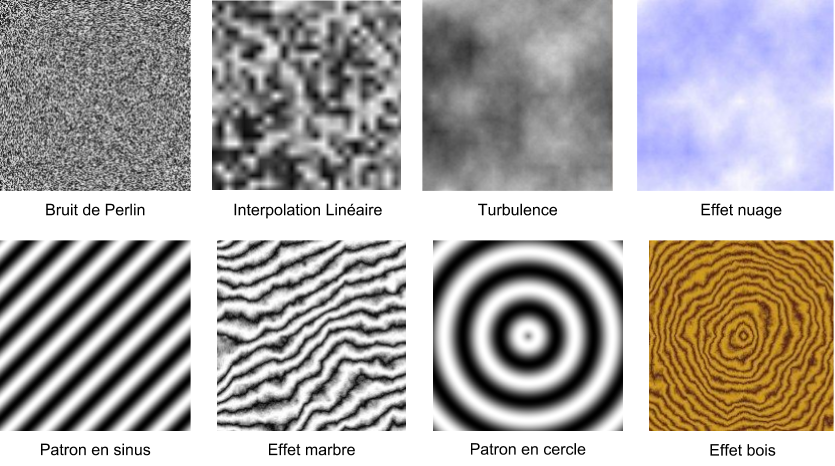
\includegraphics[width=\textwidth]{img/infog-image-procedural-texture.png}
\caption{Textures procédurales}\label{fig-procedural-texture}
\end{figure}
\paragraph{} Au niveau de l'application, une classe \texttt{texelFactory} s'occupe de générer toutes les textures procédurales présentées plus-haut (\ref{fig-procedural-texture}).  Chaque textue est interfacée par une méthode permettant de transformer un buffer \texttt{ofPixels} avec des paramètres (puissance de la turbulence par exemple) qui seront utilisées par les algorithmes correspondants (réf. \ref{src-procedural-texture}). Par la suite, ce buffer est appliqué sur le \texttt{GameObject} qui possède un \texttt{ofTexture} et un \texttt{ofMesh} propre. Aussi, lors de la création du \texttt{ofMesh}, il est nécessaire de cartographier la texture sur la forme avec la méthode \texttt{ofMesh::addTextCoord} et \texttt{ofTexture::getCoordFromPercent}.
\subsection{Cubemap}